\documentclass{standalone}

\usepackage[scaled]{helvet} % Helvetica, scaled 95%
\usepackage{tikz}
\usetikzlibrary{shapes, shapes.geometric, arrows}
\usetikzlibrary{positioning}
\tikzset{every picture/.style={/utils/exec={\sffamily}, line width=0.75pt}}

\begin{document}

%\tikzset{every picture/.style={line width=0.75pt}} %set default line width to 0.75pt        

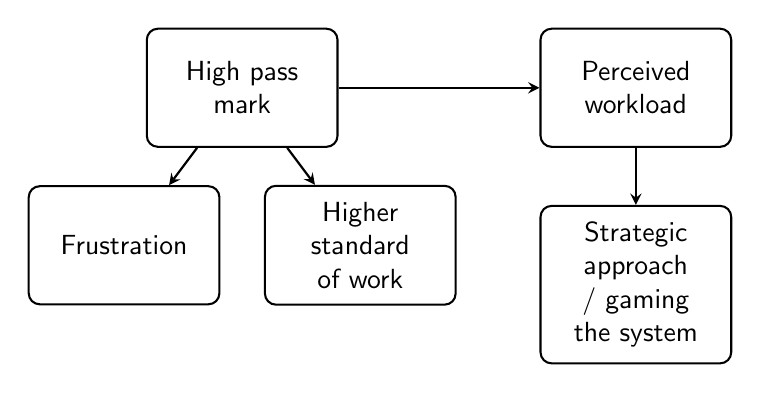
\begin{tikzpicture}[x=0.75pt,y=0.75pt,yscale=-1,xscale=1,every node/.style={theme}]

     \tikzstyle{theme} = [rounded corners,
						fill = white,
						draw = black,
						minimum width = 2cm,
						minimum height = 1.5cm,
						inner sep = 6pt,
						text centered,
						text width = 2cm,
						%xshift = 2.2cm
						]
     \tikzstyle{arrow} = [thick,->,>=stealth]

\node [] (t1) {High pass mark};
\node [on grid, below left = 2cm and 1.5cm of t1] (t1a) {Frustration};
\node [on grid, below right = 2cm and 1.5cm of t1] (t1b) {Higher standard of work};
\node [on grid, right of = t1, node distance=5cm] (t2) {Perceived workload};
\node [on grid, below of = t2, node distance=2.5cm] (t3) {Strategic approach / gaming the system};
\draw[arrow] (t1) -- (t2);
\draw[arrow] (t1) -- (t1a);
\draw[arrow] (t1) -- (t1b);
\draw[arrow] (t2) -- (t3);

\end{tikzpicture}


\end{document}